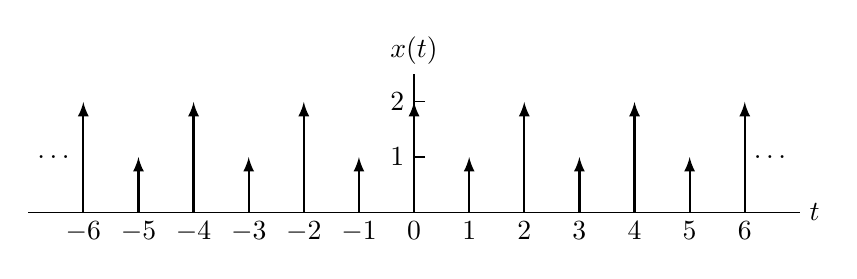
\begin{tikzpicture}[scale=0.70]
	\draw (-7,0) -- (7,0) node[anchor=west] {$t$};
	\draw (0, 0) -- (0,2.5) node[anchor=south] {$x(t)$};	
	\foreach \x in {-6, -5, ..., 6}
	{
		\draw (\x, 0.2) -- ++(0, -0.2);
		\node at (\x, 0) [anchor=north ] {$\x$};
	}
	\foreach \y in {1,2}
	{
		\draw (0.2, \y) -- ++(-0.2, 0);
		\node at (0, \y) [anchor=east ] {$\y$};
	}	
	
	\foreach \x in {-6, -4, ..., 6}
	{
		\draw[thick, latex-] (\x, 2) -- ++(0, -2);
	}
	
	\foreach \x in {-5, -3, ..., 5}
	{
		\draw[thick, latex-] (\x, 1) -- ++(0, -1);
	}	
	
	\node at (-6.5, 1) {\dots};
	\node at (6.5, 1) {\dots};
	
\end{tikzpicture} 